\newcommand{\bitmap}{\proc{bmap}}
\newcommand{\pcounting}{\proc{Contagem Probabilística}}
\newcommand{\pc}{\proc{ProbabilisticCounting}}
\newcommand{\pcpp}{\proc{ProbabilisticCounting{+}{+}}}

\chapter{Contagens Probabilísticas}
\label{lab:flajolet-martin}

Na seção anterior, abordamos a solução de Morris para o problema da contagem aproximada, que tinha como objetivo 
principal, reduzir o espaço utilizado para se manter a quantidade de elementos de um conjunto dado. Os fatos de, no 
contexto vivenciado por Morris, não ser possível armazenar o conjunto todo nem manter a contagem em uma variável por 
conta de não existirem máquinas com registradores maiores que 8 bits tornam esse problema interessante. 

Contudo, no contexo atual, em que os programas têm a disposição inteiros de 32 bits ou 64 bits, o problema da contagem
aproximada parece não ser relevante. A razão disso é que o custo para mantermos um simples contador é praticamente nulo 
nos dias atuais, de modo que, uma solução probabilística não seria tão benéfica do ponto de vista do consumo de memória.
Mesmo que esse problema não tenha aplicações imediatas atualmente, a solução proposta por Morris contém aspectos que 
inspiraram soluções de problemas mais desafiadores. Um desses problemas é descobrir o número aproximado de elementos 
distintos em um fluxo de dados~$\Mbb$. 

\begin{quote}
  \textbf{Problema} da \proc{ContagemDistintaAproximada($\Mbb$, $k$):} Dado um fluxo de dados com repetições
  $\Mbb = \{ x_1, x_2, \dots, x_s, \dots \}$, \textbf{encontrar} estimador $\hat{n}$ para o número~$n$ de elementos 
  \textit{distintos} de $\Mbb$ usando não mais que $k$ bits.
\end{quote}

Um modo de encontrarmos \textit{exatamente} a quantidade de elementos distintos de~$\Mbb$ é inserir cada item novo que 
for aparecendo em um tabela e assim, o tamanho desta tabela será a resposta para o problema. A fragilidade dessa solução 
é o consumo de memória proporcional ao número de elementos distintos, e isto pode ser uma grande limitação em situações 
nas quais existam vários fluxos sendo monitorados. 

\textit{Reddit} é um site que tem como principal funcionalidade a criação de grupos de discussões, nos quais usuários 
podem expor suas opiniões sobre um dado tema. E um dos desafios enfrentados por esse site é manter o número de 
visualizações distintas de cada grupo~\citep{Reddit}. Nessa situação, em que existem milhões de grupos e cada um podendo 
ter milhares ou milhões de visualizações, manter uma tabela para cada discussão armazenando um indentificador dos 
usuários que a visualizaram seria uma solução muito custosa. Outro fato agravante é que a quantidade de visualizações 
distintas é basicamente um número, mas teríamos que gastar espaço proporcional a este valor para mantermos esse número 
corretamente.

Em muitos casos, não precisamos do valor \textit{exato} da quantidade de elementos distintos em $\Mbb$. Podemos assim, 
tentar projetar algoritmos \textit{aproximados} e que consomem muito menos memória. Uma das primeiras soluções para o 
problema da contagem distinta aproximada foi elaborada por \textit{Philippe Flajolet} e \textit{Nigel Martin}
~\citep{flajolet:martin:85}. A motivação inicial desses autores era otimizar pesquisas em banco de dados relacionais, e 
a principal dificuldade nesse processo era calcular o número de elementos distintos em uma coluna. Nas próximas seções, 
veremos o algoritmo desenvolvido por Flajolet e Martin, conhecido como \proc{Contagem Probabilística}.

\section{Algoritmo da \proc{Contagem Probabilística}}
\label{sec:flajolet-martin:algorithm}

O algoritmo da \proc{Contagem Probabilística} supõe a existência uma função de hash~$h$ que associa uniformemente cada 
elemento do fluxo $\Mbb$ para um número inteiro entre $0$ e $2^L-1$ inclusive, em que $L$ é a quantidade necessária de 
bits para mapear todas as entradas de~$\Mbb$. O algoritmo também utiliza a função $\rho$ que recebe um inteiro $y$ de 
$L$ bits e devolve a posição indexada do zero do dígito menos significativo da representação binária de $y$. Vamos ver 
exemplos para $L = 4$. Temos que $\rho(12) = \rho(1100_2) = 2$ e $\rho(9) = \rho(1001_2) = 0$. Um caso particular é 
quando $y = 0$ e nesta situação, $\rho(0) = L$. E teremos um vetor $\bitmap$ de tamanho $L + 1$ inicializado com zeros.

Assim, para cada $x_i$ em $\Mbb$, cacularemos um inteiro $y_i \coloneqq h(x_i)$. Em seguida, encontraremos o valor de 
$\rho(y_i)$ e setaremos a posição $\rho(y_i)$ do vetor $\bitmap$ para $1$. Dessa forma, esse vetor guardará quais valores 
$\rho(h(x_i))$ aparecem no fluxo $\Mbb$.

Por fim, seja $R$ o menor índice tal que $\bitmap[R] = 0$. A estimativa para o número de elementos distintos de 
$\Mbb$ será $2^R/\phi$, em que, $\phi$ é um fator de correção cujo valor é $0.77351{\dots}$ e cuja origem pode ser vista
detalhadamente em ~~\citep{flajolet:martin:85}.

Vamos ver um exemplo de execução do algoritmo descrito acima. Considere que $\Mbb = \{ 4, 6, 8, 6, 9, 14 \}$, $L = 4$ e
que a função $h$ é a identidade, ou seja, para todo $x_i$, temos que $h(x_i) = x_i$. Na primeira iteração, $x_1 = 4$ e 
$\rho(4) = \rho(0100_2) = 2$. Assim, setamos $\bitmap[2] = 1$. Agora, na segunda iteração, 
$\rho(x_2) = \rho(6) = \rho(0110_2) = 1$, e setamos $\bitmap[1] = 1$. Na terceira iteração, temos que 
$\rho(x_3) = \rho(8) = \rho(1000_2) = 3$ e portanto, $\bitmap[3] = 1$. Na quarta iteração, o elemento $6$ já apareceu, 
então $\bitmap$ permanece intacto. Na iteração seguinte, $\rho(x_6) = \rho(9) = \rho(1001_2) = 0$ e $\bitmap[0] = 1$.
Na última iteração, $\rho(x_7) = \rho(14) = \rho(1110_2) = 1$, mas a posição 1 de $\bitmap$ já esta setada e dessa forma,
$\bitmap$ permance o mesmo. Falta, por fim, encontrar o valor de $R$. Como as posições 0, 1, 2, e 3 de $\bitmap$ estão
preenchidas, temos que $R = 4$ e que a estimativa do número de elementos distintos de $\Mbb$ é 
$2^{R}/\phi = 2^4/0.77351 \approx 21$. A estimativa anterior está muito distante do valor real, que é $5$. Nas seções
seguintes verificaremos se essa situação se repete para fluxos com muito mais elementos.

O algoritmo $\pc$ a seguir recebe um fluxo $\Mbb = \{ x_1, x_2, \dots, x_s, \dots \}$ com $n$ elementos distintos, 
um inteiro $L$ que representa quantos bits o algoritmo consumirá e uma função de hash~$h$ que mapeia os elementos $\Mbb$ 
para inteiros entre $0$ e $2^L - 1$ inclusive. E esse algoritmo devolve estimador $\hat{n}$ para $n$ da forma 
$2^{R}/\phi$, em que, $R$ é um número inteiro e $\phi$, uma constante teórica. Veremos mais adiante que 
$\Ebb(R) = \lg \phi n$, $\phi = 0.77351{\dots}$ e $\sigma(R) = 1.12$.

\begin{codebox}
  \Procname{$\pc(\Mbb, h, L)$}
  \li \For i de $0$ até $L + 1$
      \Do
  \li    $\bitmap[i] \gets 0$
      \End
  \li \For cada $x$ em $\Mbb$                               \label{li:pc:for:start}
      \Do
  \li   $y \gets h(x)$
  \li   $\bitmap[\rho(y)] \gets 1$                          \label{li:pc:for:end}
      \End
  \li $R \gets \{ \min 0 \leq i \leq L: \bitmap[i] = 0 \}$  \label{li:pc:r:def}
  \li\Return $2^R/\phi$
  \End
\end{codebox}

\section{Padrões nos bits}
\label{sec:flajolet-martin:pattern}

Na seção anterior, descrevemos o algoritmo da \proc{Contagem Probabilística}. Vamos, agora, tentar entender a intuição
por trás dessa solução.

No algoritmo $\pc(\Mbb, h, L)$, a função~$h$ que mapeia uniformemente os elementos do fluxo $\Mbb$ para inteiros entre 
$0$ e $2^L - 1$ inclusive nos permite supor que o fluxo $\Mbb$ é na verdade um fluxo de números inteiros no intervalo 
$[0, 2^L - 1]$. Nesse sentido, podemos considerar um fluxo $\Mbb_h = \{ h(x_1), h(x_2), \dots, h(x_s), \dots \} = 
\{ y_1, y_2, \dots, y_s, \dots \} $, em que $x_1, x_2, \dots$ são elementos de $\Mbb$.

Dessa forma, um elemento $y_i$ de $\Mbb_h$ pode ser visto como uma palavra binária aleatória de $L$ bits em que cada bit 
é gerado independentemente com probabilidade $1/2$. Com esta interpretração, a função $\rho$ agrupa essas palavras de 
$L$ bits de acordo com seus prefixos. Assim, as palavras $z_0$ tais que $\rho(z_0) = 0$ são aquelas cujo primeiro dígito 
é~1 ou tem prefixo da forma $0^01$. Já as palavras $z_1$ tais que $\rho(z_1) = 1$ são aquelas cujo segundo dígito é o 
menos significativo ou tem prefixo da forma $0^11$. As palavras aleatórias de $L$ bits podem, portanto, ser divididas em 
grupos de acordo com prefixos da forma $0^{*}1$.

Se os bits de uma palavra aleatória são gerados independentemente e uniformemente, então a probabilidade de uma palavra
ter um prefixo da forma $0^{k-1}1$ é $1/2^{k}$. Probabilidade e Contagem são áreas da Matemática muito relacionadas, de 
modo que ao invés de nos perguntarmos qual a probabilidade de uma palavra ter um prefixo da forma $0^{k-1}1$, podemos 
nos questionar quantas palavras tem esse prefixo. Neste caso, $1/2^{k}$ das palavras terão esse prefixo.

Assim, para um fluxo $\Mbb_h$ com $n$ elementos distintos, é possível se perguntar quantos destes elementos começam com
o dígito 1. A resposta para esta pergunta é que \textbf{esperamos} que $n/2$ palavras desse fluxo se iniciem com o 
dígito 1. E $n/2^2 = n / 4$ palavras devem ter o prefixo $0^{2-1}1 = 01$. Da mesma maneira, $n/2^3 = n/8$ palavras devem 
possuir um prefixo da forma $0^{3-1}1 = 001$. O vetor $\bitmap$, desse modo, armazena quais prefixos já apareceram no 
fluxo $\Mbb_h$. Falta, agora, entender o papel da variável $R$.

Suponha que $R = 4$, ou seja, $\bitmap[R] = 0$ e para $0 \leq i < R$, $\bitmap[i] = 1$. Vamos usar a ideia vista acima
para tentar estimar o número de elementos distintos que devem ter aparecido. Esperamos que $1/2$ dos elementos de 
$\Mbb_h$ se iniciem com o dígito 1, logo, a cada dois elementos sorteados ao acaso de $\Mbb_h$, pelo menos um deve 
começar com 1. Em outras palavras, devem ter aparecido pelos menos duas palavras para que $\bitmap[0] = 1$. Vamos ver se 
esse raciocínio faz sentido para $\bitmap[1] = 1$. O esperado é que $1/4$ dos elementos de $\Mbb_h$ comecem com $01$, 
que a cada quatro palavras sorteadas de $\Mbb_h$, pelo menos uma comece com $01$ e assim, devem ter aparecido quatro 
palavras para que $\bitmap[1] = 1$. Analogamente, devem ter aparecido pelo menos 8 palavras para que $\bitmap[2] = 1$ e 
16 palavras para que $\bitmap[3] = 1$. Como $\bitmap[R = 4] = 0$, então ainda não devem ter aparecido $32$ palavras no 
fluxo $\Mbb_h$. Portanto, a melhor estimativa nesse caso é afirmar que $\Mbb_h$ possui $2^R = 16$ elementos distintos. 

A ideia descrita nessa seção é a base para os algoritmos que resolvem o problema da contagem distinta aproximada, e 
entendê-la ajudará a vermos a origem das soluções. Na próxima seção, serão expostas alguns aspectos da prova do 
funcionamento do algoritmo da $\pcounting$. 

\section{Qualidade da aproximação}
\label{sec:flajolet-martin:analysis}

Essa seção busca destacar as principais \textbf{etapas} da análise desse algoritmo feita por Flajolet e 
Martin~\citep{flajolet:martin:85}. Dessa forma, os detalhes técnicos de algums passos da demonstração podem ser 
explorados com mais calma a partir da leitura do artigo original. Suponha que a quantidade de elementos distintos de um 
fluxo $\Mbb$ seja $n$. O valor esperado da variável $R$ definida na linha~\ref{li:pc:r:def} do algoritmo $\pc$ é 
aproximadamente $\lg \phi n$, em que $\phi = 0.77351{\dots}$ E o desvio padrão de $R$ é em torno de $1.12$. 

O primeiro passo da análise é definir a variável aleatória $R_n$ como sendo o valor da variável $R$ ao final da execução 
do algoritmo~$\pc$ para uma entrada $\Mbb$ com $n$ elementos distintos, função de hash~$h$ e inteiro $L$. Dessa forma, o 
interesse principal da demonstração é encontrar fórmulas ou estimativas para:
\begin{itemize}
  \item $p_{n,k} = \mathbb{P}(R_n = k)$: probabilidade de uma saída de $\pc$ ser igual a $k$
  \item $q_{n,k} = \mathbb{P}(R_n \geq k)$: probabilidade de uma saída de $\pc$ ser maior ou igual a $k$
  \item $\Ebb(R_n)$: valor esperado de $R_n$
  \item $\Vbb(R_n)$: variância de $R_n$
\end{itemize}

O primeiro teorema de ~\citep{flajolet:martin:85} mostra uma fórmula \textit{exata} e \textit{discreta} para $q_{n,k}$. 
A principal idea para encontrar essa fórmula é agrupar as palavras binárias por prefixos da forma $0^k1$. Assim, 
defini-se $E_k = \{ x  \ | \ \rho(x) = k \}$, ou seja, $E_k$ é o conjunto de todas as palavras aleatórias com prefixos
iguais a $0^k1$. Da mesma forma, defini-se $K_k = \{ x \ | \ \rho(x) \geq k \}$. Em seguida, as diferentes entradas 
$\Mbb$ com $n$ elementos distintos são representadas por um polinômio:
\[ P_k^{(n)} = (E_0 + E_1 + \twodots + E_{k-1} + K_k)^n .\]

O próximo passo é tentar expandir esse polinômio usando \textit{inclusão e exclusão}, e associar uma medida 
probabilidade para $E_0, E_1, \twodots, E_{k-1}, K_k$. E a prova deste teorema termina encontrando uma relação entre 
$q_{n,k}$ e esta expansão de polinômio.

Em seguida, o Teorema 2 de~\citep{flajolet:martin:85} apresenta aproximações de $q_{n,k}$ para diferentes intervalos de 
$k$. E a consequência deste teorema é a existência de uma distribuição limitante para a distribuição de probabilidade de 
$R_n$ conforme $n$ cresce. Dessa forma, obtém-se uma fórmula \textit{aproximada} e \textit{contínua} para $q_{n,k}$:
\[ q_{n,k} \approx \psi(\frac{n}{2^k}) \]

em que, $\psi(x) = \prod_{j \geq 0} (1 - e^{-x2^j})$.

Note que por definição, $p_{n,k} = q_{n,k} - q_{n,k+1}$. Assim, pode-se aproximar $p_{n,k}$:
\[ p_{n,k} \approx \psi(\frac{n}{2^k}) - \psi(\frac{n}{2^{k+1}}) \ . \]

O interesse passa a ser, portanto, estimar $\Ebb(R_n)$ a partir dessa fórmula aproximada de $p_{n,k}$, de maneira 
que 
\[ \Ebb(R_n) = \sum_{k \geq 1} k p_{n,k} \approx \sum_{k \geq 1} k \Big[ \psi \Big( \frac{n}{2^k} \Big) - \psi 
  \Big( \frac{n}{2^{k+1}} \Big) \Big] \ . \]

Desse modo, defini-se a função real $F(x)$ como sendo
\[ F(x) =  \sum_{k \geq 1} k \Big[ \psi \Big( \frac{n}{2^k} \Big) - \psi \Big( \frac{n}{2^{k+1}} \Big) \Big] \ . \]

E o Lema 1 do artigo, afirma que 
\[ \Ebb(R_n) = F(x) + O \Big( \frac{1}{n^{0.49}} \Big) \ , \]
ou seja, que o valor esperado de $R_n$ se aproxima de $F(x)$ conforme $n$ cresce.

Em seguida, o Lema 2 apresenta o resultado da \hyperref[ap:mellin]{transformada de Mellin} de $F(X)$. A principal razão 
para se calcular essa transformação é que se pode expressar a fórmula inversa da transformada de Mellin como uma 
expansão assintótica cujos termos são resíduos da transformada. Assim, o Teorema $3A$ utiliza os Lemas 1 e 2, e o 
Teorema dos Resíduos para afirmar que 
\[ \Ebb(R_n) = \lg \phi n + P(\lg n) + o(1) \ , \]
em que, $P(x)$ é a expansão assintótica de $F(x)$ e $\phi = 0.77351{\dots}$, concluindo a prova que 
$\Ebb(R_n) \approx \lg \phi n$.

A prova para a estimativa de $\Vbb(R_n)$ segue os mesmos passos da prova anterior. Pela definição de 
\hyperref[ap:variance]{variância}, precisa-se estimar $\Ebb(R_n ^ 2)$. Assim, 
\[ \Ebb(R_n ^ 2) = \sum_{k=1} k^2 p_{n,k} \approx G(x) \ , \]
em que
\[ G(x) = \sum_{k=1} k^2 p_{n,k} \ . \]

Dessa forma, encontra-se a transformada de Mellin de $G(x)$ e se analisa a inversa desta transformação para estimar 
$\Ebb(R_n^2)$.

\section{\proc{Lei dos Grandes Números} novamente}

Na seção anterior, foi visto que $\Ebb(R_n) \approx \lg \phi n$, em que $\phi \approx 0.77351$. Assim, se o valor 
do contador $R$ no final do algoritmo~$\pc$ para uma entrada com $n$ elementos distintos for aproximadamente igual a 
$\lg \phi n$, então a saída desse algoritmo é aproximadamente $n$. A Tabela \ref{tab:flajolet} mostra que, em alguns 
casos, a saída do programa é praticamente igual a $n$ quando $R_n \approx \lg \phi n$.

\begin{center}
  \def\arraystretch{2}%
  \begin{table}
    \begin{tabular}{ |p{1.5cm}||p{2.5cm}|  }
      \hline
      \multicolumn{1}{|p{1.5cm}|}{\centering $n$ } 
      & \multicolumn{1}{|p{2.5cm}|}{\centering $2^{\lg(\phi n)} \slash \phi$}  \\
      \hline
      \multicolumn{1}{|p{1.5cm}|}{\centering 50 } 
      & \multicolumn{1}{|p{2.5cm}|}{\centering 49.99 }  \\
      \hline
      \multicolumn{1}{|p{1.5cm}|}{\centering 500 } 
      & \multicolumn{1}{|p{2.5cm}|}{\centering 500.0 }  \\
      \hline
      \multicolumn{1}{|p{1.5cm}|}{\centering 5000 } 
      & \multicolumn{1}{|p{2.5cm}|}{\centering 4999.99 }  \\
      \hline
      \multicolumn{1}{|p{1.5cm}|}{\centering 50000 } 
      & \multicolumn{1}{|p{2.5cm}|}{\centering 50000.0 }  \\
      \hline
     \end{tabular}
     \caption{\label{tab:flajolet} Comparação entre $n$ e a saída do algoritmo~$\pc$ quando $R_n \approx \lg \phi n$.}
  \end{table}
\end{center}

Contudo, $\Vbb(R_n) \approx\nolinebreak 1.12$ e consequentemente, o desvio padrão de $R_n$ é aproximadamente~$1$. 
Isto quer dizer que o valor de $R_n$ pode ser uma unidade maior ou menor que $\lg \phi n$, o que implica que a 
estimativa de $n$ possa ser duas vezes maior ou menor que $n$. Logo, o algoritmo $\pc$ apresenta uma grande 
variabilidade.

De modo similar ao que foi visto em \hyperref[sec:morris:plus]{\proc{Morris} e a \proc{Lei dos Grandes Números}}, 
podemos obter a partir do algoritmo~$\pc$, uma solução com variância menor. Assim, o algoritmo $\pc{+}$ recebe um fluxo 
de dados $\Mbb$, inteiros $m$ e $L$, além de uma lista de $m$ funções de hash $\mathbb{H}$, em que cada função 
$\mathbb{H}_i$ desse grupo mapeia uniformemente os elementos de $\Mbb$ para o intervalo $[0, 2^L - 1]$. Esse algoritmo 
modificado manterá $m$ vetores $\bitmap$, de maneira que para cada elemento $x$ de $\Mbb$, para todo $0 \leq j < m$, 
vamos setar $\bitmap_j[\rho(\mathbb{H}_{j}(x))] = 1$. Quando todos os itens de $\Mbb$ forem percorridos, calcularemos 
$R_j = \{ \min 0 \leq i \leq L: \bitmap_{j}[i] = 0 \}$ para todo $0 \leq j < m$ e em seguida, encontraremos a média 
desses valores obtendo $\bar{R}$. Por fim, a estimativa para o número de elementos distintos em $\Mbb$ será 
$2^{\bar{R}} / \phi$. 

Uma outra forma de vermos essa solução é que estamos executando em pararelo $m$ funções $\pc$ e para isso, temos que 
passar uma função de hash diferente para cada execução, a fim de produzir vetores $\bitmap$ diferentes ao final.

\begin{codebox}
  \Procname{$\pc{+}(\Mbb, \mathbb{H}, L, m)$}
  \li \For $j$ de $0$ até $m$
      \Do
  \li    \For $i$ de $0$ até $L + 1$
          \Do
  \li       $\bitmap_{j}[i] \gets 0$
          \End
      \End
  \li \For $j$ de $0$ até $m$
      \Do
  \li    \For cada $x$ em $\Mbb$
          \Do
  \li       $y \gets \mathbb{H}_{j}(x)$
  \li       $\bitmap_j[\rho(y)] = 1$
          \End
      \End
  \li \For $i$ de $0$ até $m$
      \Do
  \li    $\mathbb{R}[j] = \{ \min 0 \leq i \leq L: \bitmap_{j}[i] = 0 \}$
      \End
  \li $\bar{R} = \sum_{j=0}^{m} \mathbb{R}[j] / m$
  \li \Return $2^{\bar{R}}/\phi$
  \End
\end{codebox}

Seja $\bar{R_n}$ o valor da variável $\bar{R}$ ao final da execução do algoritmo~$\pc{+}$ para uma
entrada com $n$ elementos distintos. De forma análoga aos resultados vistos em \hyperref[sec:morris:plus]{\proc{Morris} 
e a \proc{Lei dos Grandes Números}}, pode-se concluir que:
\[ \Ebb(\bar{R_n}) \approx \lg \phi n   \; \; \text{e}  \; \; \Vbb(\bar{R_n}) \approx \frac{1.12}{m} \ . \]

No entanto, o fato de precisarmos de uma função de hash distinta para cada iteração torna a solução acima inviável, uma 
vez que, encontrar funções que mapeiem na prática os elementos de um conjunto $\Mbb$ de maneira uniforme não é uma 
tarefa simples. Para contornar esse problema, os autores propuseram o uso da \textbf{média estocástica}.

Essa ideia consiste em dividr os elementos da entrada em $m$ lotes e usar parte da informação do hash dos elementos para 
definir em qual lote um elemento deve ir. As linhas \ref{li:pcpp:for:start}-\ref{li:pcpp:for:end} do algoritmo~$\pc{++}$ 
a seguir mostram como essa divisão é feita.

\begin{codebox}
  \Procname{$\pc{++}(\Mbb, $h$, $L$)$}
  \li \For $j$ de $0$ até $m$
      \Do
  \li    \For $i$ de $0$ até $L + 1$
          \Do
  \li       $\bitmap_{j}[i] \gets 0$
          \End
      \End
  \li \For cada $x$ em $\Mbb$                                                         \label{li:pcpp:for:start}
      \Do
  \li   $\texttt{lote} \gets h(x) \mod k$
  \li   $y \gets \lfloor h(x) / k \rfloor$
  \li   $\bitmap_{\texttt{lote}}[y] = 1$                                              \label{li:pcpp:for:end}
      \End
  \li \For $i$ de $0$ até $m$
      \Do
  \li    $\mathbb{R}[j] = \{ \min 0 \leq i \leq L: \bitmap_{j}[i] = 0 \}$             \label{li:pcpp:rmin}
      \End
  \li $\bar{R} = \sum_{j=0}^{m} \mathbb{R}[j] / m$
  \li \Return $m \times 2^{\bar{R}}/\phi$
  \End
\end{codebox}

Se a função de hash $h$ distribuir os $n$ elementos distintos do conjunto $\Mbb$ uniformemente entre os $m$ lotes, então 
esperamos que cada lote tenha aproximadament $\frac{n}{m}$ elementos. Nesse caso, $2^{\bar{R_n}}/\phi$ seria uma 
aproximação para $\frac{n}{m}$. É devido a este fato que a saída do algoritmo~$\pc{++}$ é 
$\mathbf{m} \times 2^{\bar{R_n}}/\phi$, pois este valor é uma estimativa para $\mathbf{m} \times \frac{n}{m} = n$.

Por fim, o erro relativo esperado do algoritmo \pcpp é em torno de $0.78 / \sqrt{m}$. Isto quer 
dizer que para $m = 64$, o desvio esperado é em torno de $10\%$. Dessa forma, a escolha de $m$ depende das exigências do 
problema. Se precisarmos de uma precisão maior, escolheremos um valor de $m$  maior, mas teremos um algoritmo mais 
custoso em termos de tempo e espaço. Por outro lado, se a exigência é, por exemplo, decidir qual de dois conjuntos tem a 
menor quantidade de elementos distintos, podemos escolher um valor menor de $m$ para fazer essa comparação, mesmo tendo 
um risco maior de escolher o conjunto errado.

\section{Estimando valores pequenos com a \proc{Contagem Probabilística}}
\label{sec:fm:low_estimates}

Uma das principais razões para escolhermos algoritmos \textit{probabilísticos} ao invés de algoritmos \textit{exatos} é 
o \textbf{consumo de memória reduzido}. Como já foi abordado, para resolver o problema da contagem distinta de forma 
\textit{exata}, podemos manter uma tabela de hash e conforme os elementos forem processados, adicionar a esta tabela 
somente aqueles elementos que não apareceram ainda. Assim, a quantidade de elementos distintos processados será o tamanho 
da tabela. Suponha que cada hash seja um inteiro de 4 bytes (32 bits) e que existam um milhão de itens distintos 
percorridos. Para armazenar essa tabela, gastaríamos pelos menos 4 MB. Por outro lado, se usarmos o algoritmo da
$\pcounting$ para resolver esse problema, o consumo de memória seria proporcional ao valor $m$ e não dependeria da 
quantidade de itens distintos. Logo, se o vetor $\bitmap$ for um vetor de inteiros de 4 bytes de tamanho $m$, e 
$m$ for igual a 1024, então a memória consumida por esse algoritmo seria em torno de 4 KB, que é um consumo de espaço
\textbf{1000 vezes menor} que a solução exata.

O erro relativo esperado da $\pcounting$ para $m = 1024$ é em torno de $2{,}5\%$. Logo, para um fluxo de milhões de 
itens distintos, o erro seria em torno das dezenas ou centenas de milhares. Com esse tipo de desvio, teríamos como 
mensurar a ordem de grandeza do número de itens distintos que já passaram pelo fluxo com bastante confiança. Contudo, 
para utilizar a $\pcounting$, o viés desse algoritmo deve ser entendido.

O \textbf{viés} de um estimador é a diferença entre seu valor esperado e o valor real do parâmetro estimado. 
Nesse sentido, a estimativa da quantidade de elementos em um conjunto devolvida pelo algoritmo de \proc{Morris} é 
\textit{não-viesada}, uma vez que, o \hyperref[morris:theorem:expected_value]{Teorema do valor esperado de $\Morris$} 
afirma que o valor esperado deste estimador é igual ao tamanho do conjunto estimado.

Na prova descrita em ~\citep{flajolet:martin:85}, o estimador de $\lg n$ é $R_n$, que representa o valor da variável 
$R$ ao final da execução de \proc{ProbabilisticCounting}, tendo como entrada um fluxo de dados com $n$ elementos 
distintos. Vimos que o valor esperado de $R_n$ é aproximadamente $\lg \phi n$, que é diferente de $\lg n$. Portanto, 
$R_n$ é um estimador \textit{viesado} de $\lg n$. E analogamente, o estimador devolvido por \pcpp também é 
\textit{viesado}.  

Então, além do erro padrão, existe também o viés do algoritmo da \proc{Contagem Probabilística}, cujo valor é 
$1 + 0{,}31/m$. Contudo, para valores de $m$ maiores que $32$, o viés se torna desprezíval se comparado ao erro padrão. 
Dessa forma, uma pessoa pode ser induzida a concluir que a escolha de $m$ é o único cuidado que ela deve tomar ao 
utilizar esse algoritmo. No entanto, ainda existe o problema de estimar \textbf{baixas cardinalidades} com essa 
estrutura.

Suponha, portanto, que $m = 64$ e que o hash do único elemento que já passou por um fluxo $\Mbb$ comece com $1$. Logo, 
se passarmos $\Mbb$ para \pcpp, existiria um vetor $\bitmap$ cuja primeira posição teria o valor $1$, e o restante dos 
vetores $\bitmap$ teriam todos valores zero. Assim, $\bar{R}$ seria igual a $1/64$, e o estimador de $n$ teria o valor 
de $64 \ 2^{\frac{1}{64}}/\phi \approx 83.64$. Esta estimativa está muito distante do valor real, que é $n = 1$.

Em vista disso, um tratamento especial deve ser dado para situações em que a cardinalidade do número de elementos 
distintos de um conjunto for baixa. Poderíamos, por exemplo, manter os elementos percorridos em uma tabela de hash, e 
quando essa tabela atingisse um certo tamanho, passaríamos a usar a estratégia original da $\pcounting$, que é preencher
os vetores $\bitmap$.  

O artigo ~\citep{flajolet:martin:85} nomeia esse problema como \textbf{não-lineariade inicial}, e os autores afirmam que 
a estimativa se aproxima do valor esperado do estimador assim que a quantidade de elementos distintos atinge pelo menos 
os valores $10m{-}20m$. Assim, para $m = 64$, é esperado que essa imprecisão inicial desapareça quando aproximadamente 
$600{-}1200$ dados distintos passarem pelo fluxo.

Vale lembrar, no entanto, que a proposta inicial para a adoção de estruturas de dados probabilísticas é o alto consumo 
de memória conforme o volume dos dados cresce. Nesse sentido, esse problema da não-linearidade inicial pode ser 
desconsiderado dependendo da situação. 

\section{Um, dois, três, \dots, repetido, \dots}
\label{sec:fm:experiments}

Nesta seção, apresentaremos a implementação da $\pcounting$. Além disso, experimentos similares ao da 
Seção~\ref{chap:morris:experiments} forams realizados com o objetivo de se verificar a acurácia dessa solução.

A implementação foi baseada no algoritmo $\pcpp$ com algumas modificações. Dessa forma, definimos uma 
classe~\texttt{ProbabilisticCounting}, cujo construtor recebe os parâmetros $m$ e $L$. E nesta classe, existem os 
métodos \texttt{adiciona} e \texttt{conta}. O primeiro adiciona um elemento à estrutura, e o segundo devolve a 
estimativa da quantidade de elementos distintos. Dessa forma, as simulações se baseiam em uma versão \textit{online} da 
$\pcounting$ para que possamos observar como a estimativa evolui conforme novos itens são inseridos nessa estrutura.

\begin{lstlisting}[style=mypython,caption=Implementação do algoritmo $\pc$,captionpos=b, label=pc:code]
class ProbabilisticCounting:
    def __init__(self, m=64, L=64):
        self.m: int = m
        self.L: int = L
        self.phi = 0.77351
        self.BITMAP: List[List[int]] = []

        for _ in range(0, self.m):
            self.BITMAP.append([None] * self.L)

        self.R: List[int] = [0] * self.m
        self.R_sum = 0

    def p(self, x: int):
        return (x & -x).bit_length() - 1

    def adiciona(self, x: int):
        lote = x % self.m
        y = x // self.m
        self.BITMAP[lote][self.p(y)] = 1

        while self.BITMAP[lote][self.R[lote]] == 1:
            self.R[lote] += 1
            self.R_sum += 1

    def conta(self):
        R = self.R_sum / self.m

        return floor((self.m * pow(2, R)) / self.phi)
\end{lstlisting}

Vamos comentar alguns detalhes de implementação do Programa~\ref{pc:code}. O primeiro deles é relacionado ao método
~\texttt{adiciona}, que foi baseados nas linhas~\ref{li:pcpp:for:start}--\ref{li:pcpp:rmin} do algoritmo~$\pcpp$. O 
principal diferencial da implementação desse método na classe~\texttt{ProbabilisticCounting} é que já mantemos o menor
valor de $R$ de cada lote atualizado, como pode ser visto no \texttt{while}. Dessa forma, a complexidade de se adicionar
um elemento nessa estrutura é $O(1)$ amortizado.

O próximo comentário é relacionado ao método \texttt{p} da classe \texttt{ProbabilisticCounting}, que é a implementação 
da função $\rho$ do algoritmo~$\pcpp$. Essa função deve retornar a posição do bit menos significativo de um inteiro. 
Assim, dado um inteiro~$x$, tentaremos encontrar uma forma de encontrar o índice do bit menos significativo de $x$. É 
interessante, portanto, considerar o oposto de $x$, ou seja, $-x$. Considerando a representação binária de $x$, $-x$ 
pode ser calculado da seguinte maneira: $\overline{x} + 1$, em que $\overline{x}$ é o complementar de $x$, cuja 
representação binária inverte todos os bits de $x$. Tendo $-x$ em mãos, a posição do único bit ligado de 
$x \ {\&} \ {-x}$ coincide com a posição do bit menos significativo de~$x$. Para recuperar esse bit, usamos a função 
\texttt{bit\_length} do \proc{Python} que retorna a menor quantidade de bits para se representar um inteiro. Esta função 
é indexado a partir do 1 e, por isso, subtraímos 1 do retorno dela. 

Vamos ver alguns exemplos para deixar esse ideia mais clara. Tome $\rho(10) = \rho(110_2) = 1$. Para chegar nesse valor 
de 1, primeiro encontramos $-10 = \overline{10} + 1 = 001_2 + 001_2 = 010_2$. Em seguida, calculamos
$10 \ {\&} \ -10 = 110_2 \ {\&} \ 010_2 = 010_2$. E a posição do único bit ligado deste número binário é 1. Outro 
exemplo é $\rho(9) = \rho(101_2) = 0$. Assim, $-9 = \overline{9} + 1 = 101_2 + 001_2 = 110_2$, e 
$9 \ {\&} \ -9 = 101_2 \ {\&} \ 110_2 = 001_2$. E o único bit ligado deste número está na posição zero, que coincide com
o valor de $\rho(9)$.

Outro detalhe de implementação é que não estamos utilizando a função de hash~$h$ durante a inserção dos elementos na 
estrutura, uma vez que, os elementos inseridos já são inteiros, e estamos supondo que eles são gerados uniformente. 
Assim, não há a necessidade de mapeá-los para inteiros entre $0$ e $2^{L} - 1$. Ou seja, implicitamente, temos que $h$ é 
a função identidade.

Tendo esclarecido os detalhes de implementação do Programa~\ref{pc:code}, podemos partir para a apresentação dos 
experimentos. O valor de $L$ utilizado nesses experimentos foi de $64$, uma vez que, a maior parte das linguagens de 
programação suporta atualmente inteiros de $8$~bytes. Além disso, gerar número aleatórios de 64 bits garatem uma maior
variabilidade dos dados dos experimentos. Outro fato importante de se destacar é que cada experimento foi repetido duas 
vezes, uma vez utilizando uma estrutura \texttt{ProbabilisticCounting} com $m = 64$ e outra vez, com uma estrutura com 
$m = 1024$. A razão disso ter sido feito foi averiguar se aumentando o valor de $m$, teríamos uma melhora considerável 
na precisão.

O primeiro experimento tem como objetivo verificar a evolução da estimativa devolvida pela estrutura 
conforme mais elementos são inseridos nela. Dessa forma, foram feitas duas simulações, em que cada simulação consistiu
em gerar um milhão de inteiros aleatórios e inserí-los em uma estrutura~\texttt{ProbabilisticCounting}. Analisaremos
primeiramente as estimativas da estrutura com $m = 64$. O gráfico da Figura~\ref{fig:pc:64:full} exibe a evolução da
estimativa devolvida pela estrutura~\texttt{ProbabilisticCounting} com $m = 64$ e podemos notar, que a estimativa, 
representada pela linha laranja, ficou um pouco distante do valor real, representado pela linha azul.

\begin{figure}[h]
  \centering
  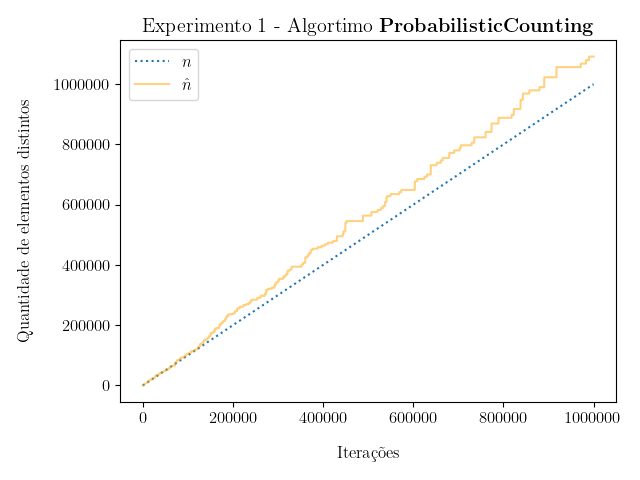
\includegraphics[height=6cm, width=\textwidth]{figuras/probabilistic_counting_full_64.png}
	\caption{Simulação do algoritmo~$\pc$ com $m = 64$ (todas as iterações)}
  \label{fig:pc:64:full}
\end{figure}

\newpage
Na Seção~\ref{sec:fm:low_estimates}, vimos que a $\pcounting$ estima pequenas cardinalidades com um grande erro. Esse 
fato pode ser confirmado na Figura~\ref{fig:pc:64:first:erro}, em que é possível perceber o erro relativo pode chegar 
até $8000\%$ logo nas primeiras iterações da simulação. A Figura~\ref{fig:pc:64:first} exibe as primeiras estimativas 
devolvidas pela estrutura~\texttt{ProbabilisticCounting}, e podemos notar que a linha das estimativas já começa distante 
da linha dos valoes reais.

\begin{figure}[h]
  \centering
  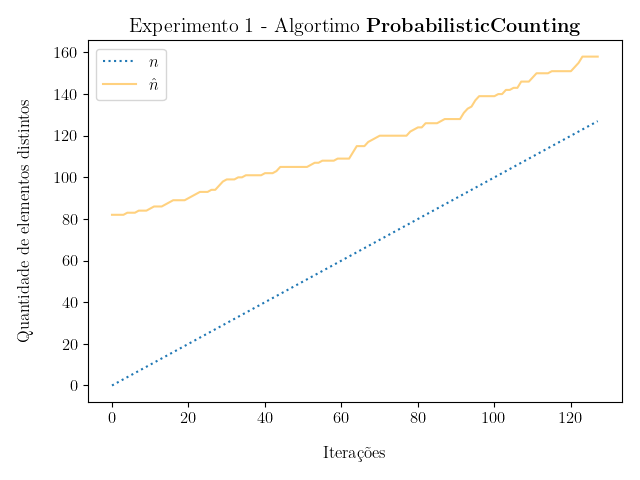
\includegraphics[height=6cm, width=\textwidth]{figuras/probabilistic_counting_first_64.png}
	\caption{Simulação do algoritmo~$\pc$ com $m = 64$ (128 primeiras iterações)}
  \label{fig:pc:64:first}
\end{figure}

\begin{figure}[h]
  \centering
  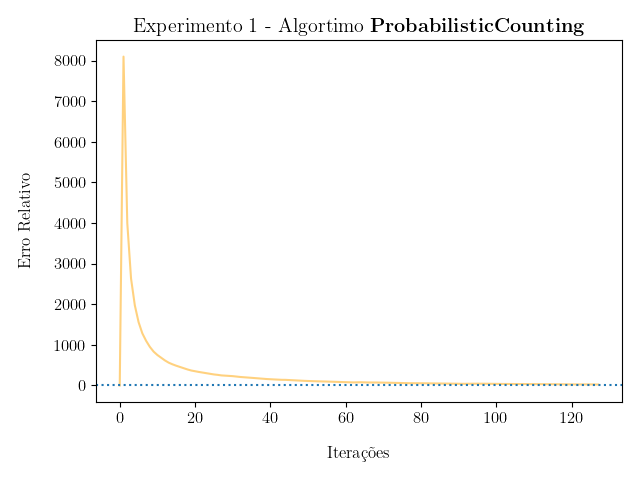
\includegraphics[height=6cm, width=\textwidth]{figuras/probabilistic_counting_erro_first_64.png}
	\caption{Erro relativo da simulação do algoritmo~$\pc$ com $m = 64$ (128 primeiras iterações)}
  \label{fig:pc:64:first:erro}
\end{figure}

\newpage
Vamos, assim, desconsiderar as primeiras iterações da simulação anterior e observar se a $\pcounting$ começa a produzir
melhores estimativas conforme mais itens são inseridos nessa estrutura. A Figura~\ref{fig:pc:64:erro:sem:first} nos 
permite concluir que nessas simulação, o problema de se estimar baixas cardinalidades desaparece após aproximadamente 
128~iterações, e depois deste ponto, os erros relativos das estimativas devolvidas ficaram dentro da faixa de erro 
esperado, que é de $10\%$, até por volta da iteração de número 150413. E dessa iteração em diante, os valores estimados 
passam a frequentemente ter um erro maior que o esperado.

\begin{figure}[h]
  \centering
  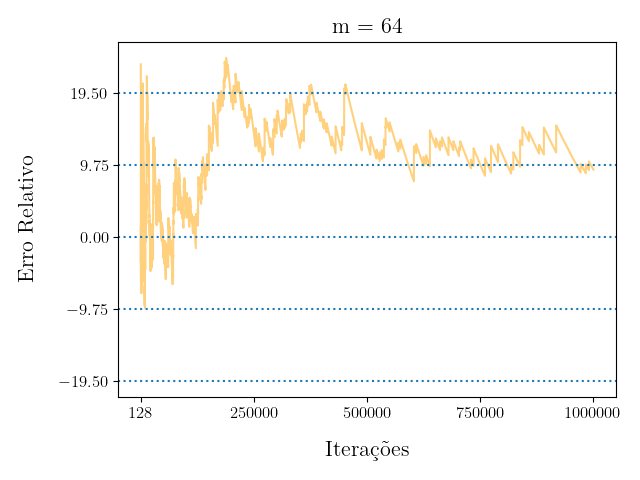
\includegraphics[height=6cm, width=\textwidth]{figuras/probabilistic_counting_erro_sem_first_64.png}
	\caption{Erro relativo da simulação do algoritmo~$\pc$ com $m = 64$ (desconsiderando asd 128 primeiras iterações)}
  \label{fig:pc:64:erro:sem:first}
\end{figure}

Dessa forma, podemos verificar se aumentando o valor do parâmetro $m$, esses problemas de precisão serão corrigidos. O 
gráfico da Figura~\ref{fig:pc:1024:full} mostra o resultado do experimento em que os mesmos elementos da simulação do 
algoritmo~$\pcpp$ com $m = 64$ foram inseridos em uma estrutura com $m = 1024$. E é possível notar que as estimativas da 
estrutura com $m = 1024$ estão bastantes próximas dos valores reais.

\begin{figure}[h]
  \centering
  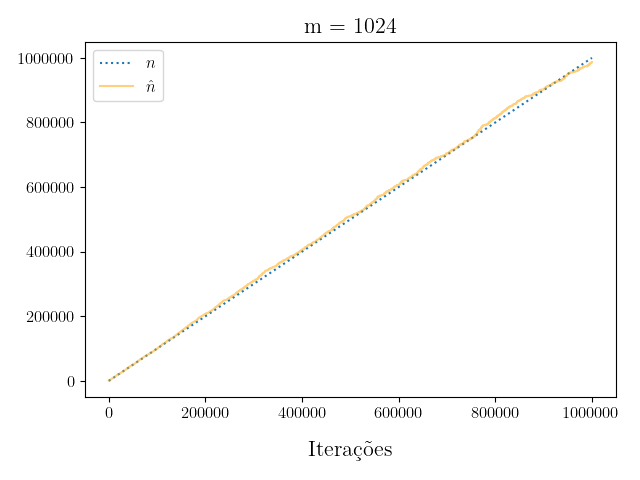
\includegraphics[height=6cm, width=\textwidth]{figuras/probabilistic_counting_full_1024.png}
	\caption{Simulação do algoritmo~$\pc$ com $m = 1024$ (todas as iterações)}
  \label{fig:pc:1024:full}
\end{figure}

\newpage
Precisamos, agora, verificar como se comportam as estimativas de baixas cardinalidades da estrutura
~\texttt{ProbabilisticCounting} com $m = 1024$. Vamos, assim, destacar as primeiras 2048 iterações da simulação 
anterior. A Figura~\ref{fig:pc:1024:first:erro}, que exibe o erro relativo nas iterações iniciais, evidencia que o erro
relativo pode chegar até $120.000\%$. E a Figura~\ref{fig:pc:1024:first}, que mostra as estimativas iniciais, reforça o 
fato que aumentar o valor de $m$ \textbf{piora} a estimativa de valores pequenos.

\begin{figure}[h]
  \centering
  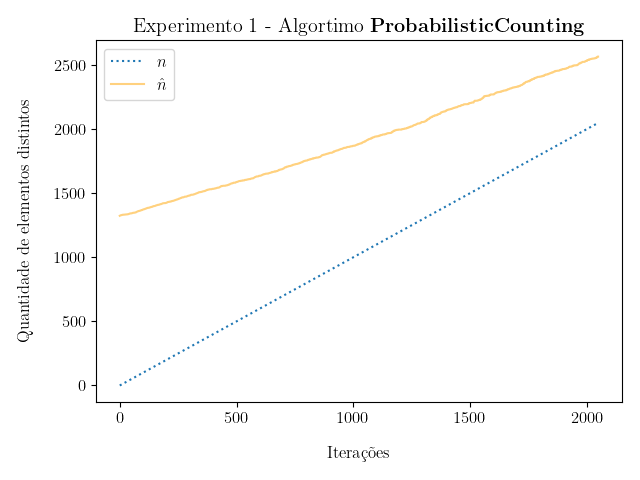
\includegraphics[height=6cm, width=\textwidth]{figuras/probabilistic_counting_first_1024.png}
	\caption{Simulação do algoritmo~$\pc$ com $m = 1024$ (2048 primeiras iterações)}
  \label{fig:pc:1024:first}
\end{figure}

\begin{figure}[h]
  \centering
  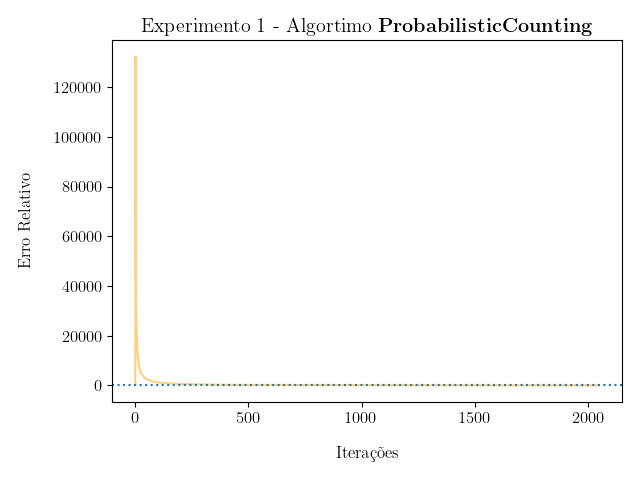
\includegraphics[height=6cm, width=\textwidth]{figuras/probabilistic_counting_erro_first_1024.png}
	\caption{Erro relativo da simulação do algoritmo~$\pc$ com $m = 1024$ (2048 primeiras iterações)}
  \label{fig:pc:1024:first:erro}
\end{figure}

\newpage
Vamos, portanto, desconsiderar as primeiras 2048 iterações da simulação anterior. A partir da observação da Figura~
\ref{fig:pc:1024:erro:sem:first}, que exibe a evolução das estimativas devolvidas pela estrutura
~\texttt{ProbabilisticCounting} desconsiderado essas iterações iniciais, podemos concluir que o erro relativo do 
algoritmo~$\pc$ ficou dentro da faixa esperada, que é de $2\%$, na maior parte da simulção. Dessa forma, se queremos 
estimar valores grandes, aumentar o parâmetro de $m$ \textbf{melhora} a precisão das estimativas.

\begin{figure}[h]
  \centering
  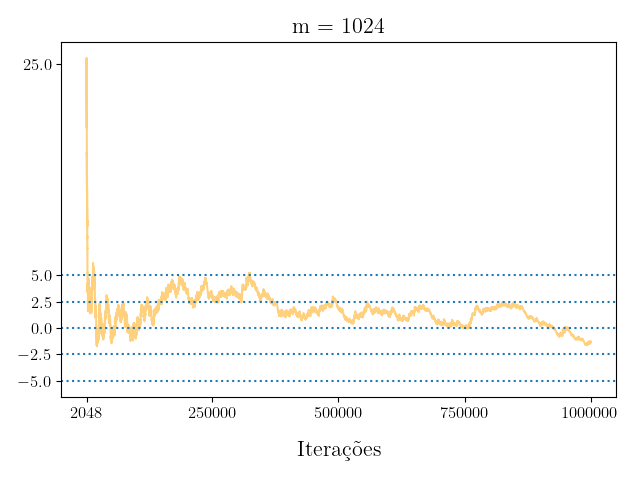
\includegraphics[height=6cm, width=\textwidth]{figuras/probabilistic_counting_erro_sem_first_1024.png}
	\caption{Simulação do algoritmo~$\pc$ com $m = 1024$ (desconsiderando as 2048 primeiras iterações)}
  \label{fig:pc:1024:erro:sem:first}
\end{figure}

% Por fim, a $\pcounting$ foi um dos primeiros algoritmos que surgiram para resolver o problema da 
% \textbf{Contagem Distinta Aproximada}, e até nos dias atuais, é uma das estruturas com o menor erro relativo esperado, 
% que é igual a $0.78 / \sqrt{m}$. Embora a $\pcounting$ não seja tão utilizado atualmente, o desenvolvimento dela serviu 
% de base para que outras estruturas com menor consumo de memória surgissem, e a análise delas é muito semelhante à 
% análise presente em ~\citep{flajolet:martin:85}. 